%%% Thesis Introduction --------------------------------------------------
\chapter{Introduction}
\ifpdf
    \graphicspath{{Introduction/IntroductionFigs/PNG/}{Introduction/IntroductionFigs/PDF/}{Introduction/IntroductionFigs/}}
\else
    \graphicspath{{Introduction/IntroductionFigs/EPS/}{Introduction/IntroductionFigs/}}
\fi

Peptides are a ubiquitous class of biological molecules which mediate key processes in living organisms. They frequently display exquisitely selective activity for their targets.\cite{craik_future_2013} This structure-dependent specificity makes them a promising target for drug development. Chemical biology in particular has benefited extensively from the development of techniques allowing access to non-native peptides.\cite{bromley_peptide_2008} Biological approaches such as recombinant peptide expression have provided some access to the material necessary for exploring protein function. However synthetic approaches allowing complete control over peptide sequence and post-translational functionalisation are fundamentally more appealing.

A synthetic approach to peptide synthesis first became practical with the introduction of solid phase peptide synthesis (SPPS) by Merrifield in the late 1960's.\cite{merrifield_solid_1963} This groundbreaking methodology allows for the construction of a native peptide backbone in a sequential, stepwise manner. This otherwise excellent technique is hampered by a limitation to sequence lengths of approximately 50 amino acid residues.\cite{dawson_synthesis_2000} Beyond this point peptide aggregation and the accumulation of truncated side products begin to stretch the limits of synthetic accessibility.

\section{Native Chemical Ligation}

The development of the Native Chemical Ligation (NCL) approach by Kent has played a major role in overcoming the length restrictions inherent to SPPS. This elegant strategy facilitates the chemoselective ligation of two unprotected peptide fragments with the formation of a native peptide bond.\cite{dawson_synthesis_1994}

\begin{scheme}[!htbp]
      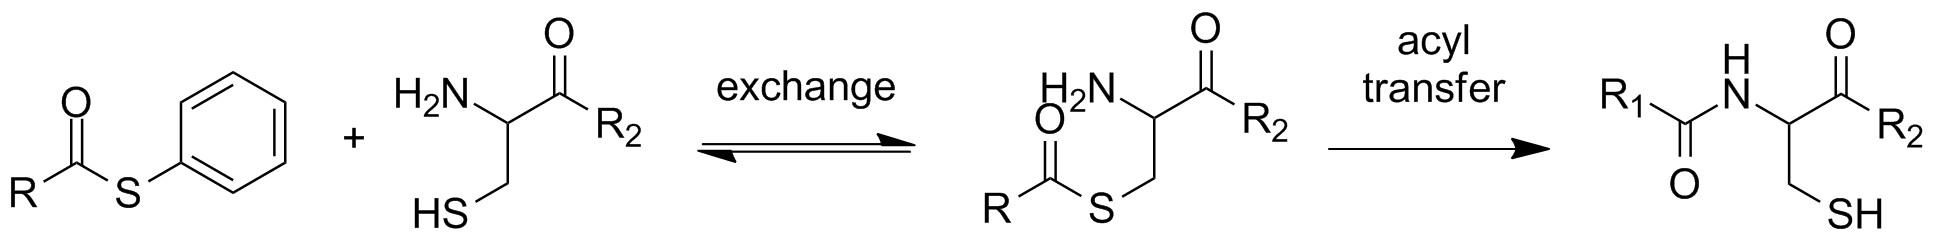
\includegraphics[width=\textwidth]{ncl.png}
      \caption{Native Chemical Ligation}
\end{scheme}

Native Chemical Ligation allows for the coupling of a C-terminal peptide thioester and an N-terminal cysteine containing peptide over two steps. In an initial Capture step the peptide thioester undergoes a bimolecular thioester exchange to form a transient thioester linked ligation product. This intermediate can subsequently undergo an irreversible intramolecular S->N acyl transfer to form a native peptide containing the desired peptide bond.

Native chemical ligation has become an indispensable tool for peptide chemists. The synthesis of biologically important peptides such as the 203 amino acid HIV-1 protease enzyme\cite{torbeev_convergent_2007} and the cyclic \textalpha-conotoxin MII \cite{clark_native_2010} exemplify this technique.

\section{Chemical Ligation at Non-Cysteine Sites}

The requirement for a cysteine residue at the ligation site in NCL is a significant limitation. The low abundance of cysteine in many proteins reduces the likelihood of finding a site amenable to NCL in the desired peptide. Extensive research efforts has been directed towards overcoming this restriction and they have been met with some significant success.

    \subsection{Auxiliary Mediated Ligation}

    Kemp and coworkers focused their attention on an NCL-like intramolecular acyl transfer approach to peptide synthesis.\cite{kemp_synthesis_1993} They developed the concept of introducing a removable thiol auxiliary at the N-terminal of the peptide (\ref{sch:auxmediatedligation}). The use of such a thiol auxiliary allows the excellent chemoselectivity of the NCL thioester exchange Capture step to be retained.

    A synthetically useful thiol ligation auxiliary should fulfill a number of criteria. It must be efficiently introducible to the N-terminal peptide, it should be compatible with solid phase peptide synthesis, it must facilitate ligation rapidly at low peptide concentrations and it must be selectively removable under mild conditions to provide a native peptide. \cite{hemantha_total_2012}

    \cmpd*{cmpd:unsubtitutedmercaptoethyl}
    \cmpd*{cmpd:methoxymercaptoethyl}
    \cmpd*{cmpd:trimethoxymercapto}

    \begin{scheme}[!htbp]
      \includegraphics[max width=\textwidth]{auxil.eps}
      \caption{General mechanism of auxiliary-mediated peptide ligation}
      \label{sch:auxmediatedligation}
    \end{scheme}

    The N\textsuperscript{\textalpha}-2-mercaptoethyl auxiliary \cmpd{cmpd:unsubtitutedmercaptoethyl} demonstrated the potential power of the auxiliary approach to creating amide bonds.\cite{canne_extending_1996} This auxiliary underwent rapid ligation and displayed a broad tolerance for many amino acids at the ligation junction. However this original auxiliary \cmpd{cmpd:unsubtitutedmercaptoethyl} was not removable from the ligated peptide.

    \begin{figure}[htbp]
      \cmpdref{cmpd:unsubtitutedmercaptoethyl}
      \cmpdref{cmpd:methoxymercaptoethyl}
      \cmpdref{cmpd:trimethoxymercapto}
      \includegraphics[max width=0.8\textwidth]{otherauxs.eps}
      \caption{A selection of previously described ligation auxiliaries}
      \label{sch:otherauxs}
    \end{figure}

    Low and coworkers further proved the utility of this approach with the total synthesis of cytochrome b562. This full-length 106 amino acid peptide was prepared from two peptide fragments via an auxiliary \cmpd{cmpd:methoxymercaptoethyl} mediated ligation at a His-Gly site.\cite{low_total_2001} Macmillan and Anderson introduced an improved acid-labile N\textsuperscript{\textalpha}-2-mercaptobenzyl auxiliary \cmpd{cmpd:trimethoxymercapto}.\cite{macmillan_rapid_2004} The trimethoxyphenyl substitution pattern increased the electron density on the ring which enhanced the acid liability of the auxiliary relative to \cmpd{cmpd:methoxymercaptoethyl}.

    The Danishefsky group employed \cmpd{cmpd:trimethoxymercapto} to good effect in the synthesis of a Human Paratyroid Hormone (hPTH) further demonstrating the synthetic utility of the auxiliary mediated ligation approach.

    \subsection{Desulfurisation Approaches to Cysteine-Free Ligation}

        An elegant alternative approach has been developed by Yan and Dawson. Their process consists of a standard NCL ligation at cysteine, followed by a desulfurisation step to yield alanine at the ligation site.\cite{yan_synthesis_2001} This extension of the NCL methodology is significant as alanine is rather more abundant than cysteine (\SI{6.3}{\percent} as opposed to \SI{1.7}{\percent}).\cite{shang_application} Yan and Dawson validated their technique with the synthesis of a 56-amino acid streptococcal protein G B1 domain.\cite{yan_synthesis_2001}

        % \begin{scheme}[h]
        %   \includegraphics[max width=\textwidth]{tcepdesulfurisation.eps}
        %   \caption[TCEP promoted desulfurisation at cysteine]{TCEP promoted desulfurisation at cysteine\cite{wan_free-radical-based_2007}}
        % \end{scheme}

        Danishefsky improved on this work by replacing Yan and Dawson's metal based thiol reduction, with a milder radical-mediated desulfurisation.\cite{wan_free-radical-based_2007} The trialkylphosphine \IUPAC{tris(2\|-carboxy\|ethyl)\|phosphine} (TCEP) promoted desulfurisation greatly simplifies post cleavage peptide isolation by eliminating the problem of peptide adsorption on the metal surface. Danishefsky has demonstrated that the TCEP promoted desulfurisation is highly selective and tolerant of the glycosyl functionalities which are ubiquitous in biological peptides.\cite{wan_free-radical-based_2007}

    \section{2-mercapto-2-phenyl Auxiliaries}

    \cmpd*{cmpd:phenylauxiliary}
    \cmpd*{cmpd:auxiliary.one}
    \cmpd*{cmpd:auxiliary.two}

    Previous work in this group has demonstrated the ability of the 2-mercapto-2-phenyl based auxiliary \cmpd{cmpd:phenylauxiliary} to participate in an auxiliary mediated ligation to provide a ligated dipeptide linked by a peptide bond. The group has also demonstrated a novel TCEP promoted cleavage of auxiliary \cmpd{cmpd:phenylauxiliary}  to yield a ligated native peptide.

    The first section of this work involves the synthesis of two acyl transfer auxiliaries \cmpd{cmpd:auxiliary.one} and \cmpd{cmpd:auxiliary.two}. It is hoped that a comparative analysis of these auxiliaries will help clarify the steric and electronic factors which influence the peptide ligation step.

    \begin{scheme}[!htbp]
      \cmpdref{cmpd:phenylauxiliary}
      \cmpdref{cmpd:auxiliary.one}
      \cmpdref{cmpd:auxiliary.two}
      \includegraphics[width=0.8\textwidth]{twoauxiliaries.eps}
      \caption{Structure of proposed ligation auxiliaries}
    \end{scheme}

    With Danishefsky's desulfurisation work in mind, we tentatively propose that a radical-mediated processes may be involved in the cleavage of this class of auxiliary. The -I inductive effects of the substituents on the proposed para substituted auxiliaries \cmpd{cmpd:auxiliary.one} and \cmpd{cmpd:auxiliary.two} should help stabilize the envisioned benzylic radical intermediate. As such we were keen to determine the effect that these substituents would have on the auxiliary cleavage process.


%%% ----------------------------------------------------------------------


%%% Local Variables:
%%% mode: latex
%%% TeX-master: "../thesis"
%%% End:
